\documentclass{IEEEcsmag}

\usepackage[colorlinks,urlcolor=blue,linkcolor=blue,citecolor=blue]{hyperref}

\usepackage{tabularx}
\usepackage{upmath}
\usepackage{amssymb}
\usepackage{amsmath}
\usepackage{array}
\usepackage{arydshln}
\usepackage{listings, multicol}
\usepackage{filecontents}
\usepackage{parcolumns}


\newcolumntype{P}[1]{>{\centering\arraybackslash}p{#1}}

\jvol{XX}
\jnum{XX}
\paper{8}
\jmonth{May/June}
\jname{Computing in Science and Engineering}
\pubyear{2021}
\newtheorem{theorem}{Theorem}
\newtheorem{lemma}{Lemma}

\setcounter{secnumdepth}{0}

\lstset{language=Python, basicstyle=\ttfamily\footnotesize}

\begin{filecontents*}{loop_fusion.py}
import numba
import numpy as np

@numba.njit(cache=True)
def loop_fusion(a):

	for i in range(10):
		a[i] += 1

	for i in range(10):
		a[i] *= 5
\end{filecontents*}

\begin{filecontents*}{parallel_multithreading.py}
import numba
import numpy as np

@numba.njit(cache=True, parallel=True)
def multithreading(a):

	for i in numba.prange(10):
		a[i] *= 10

\end{filecontents*}


\begin{document}

\sptitle{Department: Head}
\editor{Editor: Name, xxxx@email}

\title{PyExaFMM, an exercise in designing high-performance software with Python and Numba}

\author{S. Kailasa}
\affil{Department of Mathematics, University College London}

\author{T. Wang}
\affil{Department of Mechanical and Aerospace Engineering, The George Washington University}

\author{\text{L}. A. Barba}
\affil{Department of Mechanical and Aerospace Engineering, The George Washington University}

\author{T. Betcke}
\affil{Department of Mathematics, University College London}

\markboth{Department Head}{Paper title}

\begin{abstract}
    Numba is a game changing compiler for high performance computing with Python. The machine code it produces runs outside of the single-threaded Python interpreter, and can therefore fully utilize the resources of modern CPUs. This means support for parallel multithreading and auto vectorization if available, just like in a compiled language such as C++ or Fortran. Here we document our attempt to use Numba to develop a fully multithreaded implementation of the Fast Multipole Method, an algorithm which relies on a non-linear data structure and contains a significant amount of data organization that would ordinarily be run through the Python interpreter. We explain how Numba influences the design and structure of software, as well as its major pitfalls. We find that Numba doesn't live up to its promise due to overhead from the unavoidable interaction between the Python interpreter and Numba compiled code, and that our software remains an order of magnitude slower than ExaFMM-T, the leading C++ implementation of the same algorithm. However, we achieved a dramatic speedup in comparison to vanilla Python, illustrating how Numba is an excellent choice for projects in which the hackability, portability and simplicity that Python offers are a greater priorities than raw performance.
\end{abstract}

\maketitle
\chapterinitial{Python}\footnote{We use `Python' to refer to CPython, the popular C language implementation of Python, which is dominant in computational science.}, is designed for memory safety and developer productivity, not speed. Its main selling point being that it allows Computational Scientists to spend more time exploring the science, and less time being confused by strange software quirks, infuriating memory errors, and the nightmare of incompatible dependencies, all of which conspire to drain productivity when working with lower level languages.

The catch is that code is run through an interpreter and restricted to run on a single thread via a software construction called the Global Interpreter Lock [GIL]. However, libraries for high performance computational science have traditionally bypassed the issue of the GIL by using Python's C interface to call extensions built in C or other compiled languages which can be multithreaded and compiled to target special hardware features. Popular examples of this approach include Numpy and SciPy, which together have helped propel Python's popularity in computational science by providing high performance data structures for numerical data as well as interfaces for fast compiled implementations of algorithms for numerical linear algebra, and mathematical solvers for problems from differential equations to statistics and machine learning.

As the actual number-crunching itself happens outside of the interpreter, the GIL only becomes a bottleneck to performance if a program must repeatedly pass control between the interpreter and non-Python code. This is most often an issue when an optimized compiled language implementation of your desired algorithm doesn't exist in the Python Open Source, or if it requires a lot of data organization to form the input for an optimized Numpy or SciPy code, which must unavoidably take place within the interpreter. Previously, an unlucky developer would have been forced to write a compiled implementation to tackle these issues themselves and connect it to their Python package, relegating Python's role to an interface. More problematically, not all Computational Scientists have the necessary software skills or research interest in developing and maintaining complex codebases that couple multiple languages.

This is the context in which Numba was introduced \cite{Lam2015}. It is a compiler that specifically targets and optimizes Python code written with Numpy's ndarray data structure. Its power comes from the ability to generate multithreaded architecture optimized compiled code while \textit{only writing Python}. The promise of Numba is the ability to develop applications with speed that can rival C++ or Fortran, while retaining the simplicity and productivity of working in Python. We put this promise to the test by developing PyExaFMM\footnote{https://github.com/exafmm/pyexafmm}, an implementation of the particle Kernel-Independent Fast Multipole Method [FMM] \cite{Ying2004,Greengard1987}, in three dimensions. Efficient implementations of this algorithm are complicated by a recursively defined tree data structure and a series of operations which each require significant data organization and careful memory allocation. These features made PyExaFMM an excellent test case to see whether Numba could free us as Computational Scientists from the complexities of compiled languages.

We begin with an overview of Numba, focussing on when and where its use is appropriate. After introducing the necessary concepts of the FMM such as its data structure and the computations involved, we proceed with an overview of how we designed our software's data structures and API to optimally use Numba. We show how we optimized multithreaded functions for cache re-use, and discuss the main pitfalls we encountered with Numba. We conclude with two benchmarks. Firstly, we measure the impact that Numba has on vanilla Python implementations of the FMM's operators. Secondly, we demonstrate PyExaFMM's performance by comparing memory usage and runtime with ExaFMM-T \cite{Wang2021}, the leading C++ implementation of the same algorithm. We note that a strict like-for-like comparison between the two implementations isn't possible. The softwares take different approaches to the implementation of their operations and data structures. However, as the differences in the design of PyExaFMM are heavily influenced by Numba and Python, it remains useful as an illustration of what can be achieved with Python in comparison to a compiled language to solve the same problem.

\section{NUMBA}

Numba is a compiler for Python that targets a subset of the language that manipulates the $n$-dimensional array data structure from Numpy, the ndarray. Unlike a Python list, where each element is linked to the previous element by a pointer, and elements can be of any type, Numpy arrays are homogeneously typed and stored contiguously in memory.

This means that all array elements must be of the same type, and adjacent array elements are stored in adjacent memory locations. This results in two benefits for scientific computing. Firstly, modern CPUs tend to cache memory at adjacent registers when asked to load data from a given address, this is useful in algorithms which iterate over arrays as the cache is likely to contain the next element being operated on by the algorithm, saving time. This is known as \textit{locality of reference}. Secondly, the contiguous nature of the array means Numpy is able to calculate the memory addresses of sub-arrays using its knowledge of the pointer to the start of the array, the data type, and the number of elements in the slice. This is in contrast to Python lists, where subsequent element are found by following trails of pointers, known as \textit{indirection}.

Numba is built using LLVM, a tool for building custom compilers, that provides an API to generate machine code for different hardware architectures such as CPUs and GPUs. LLVM is also able to analyze the code it's compiling for hardware level optimizations such as auto vectorization. Numba doesn't replace the Python interpreter, instead  functions are marked for Numba compilation with a decorator (see listings (\ref{code:loop_fusion}) and (\ref{code:parallel_multithreading})), and when called at runtime compiled on the fly, as illustrated in figure (\ref{fig:numba}).

\begin{figure*}
    \centerline{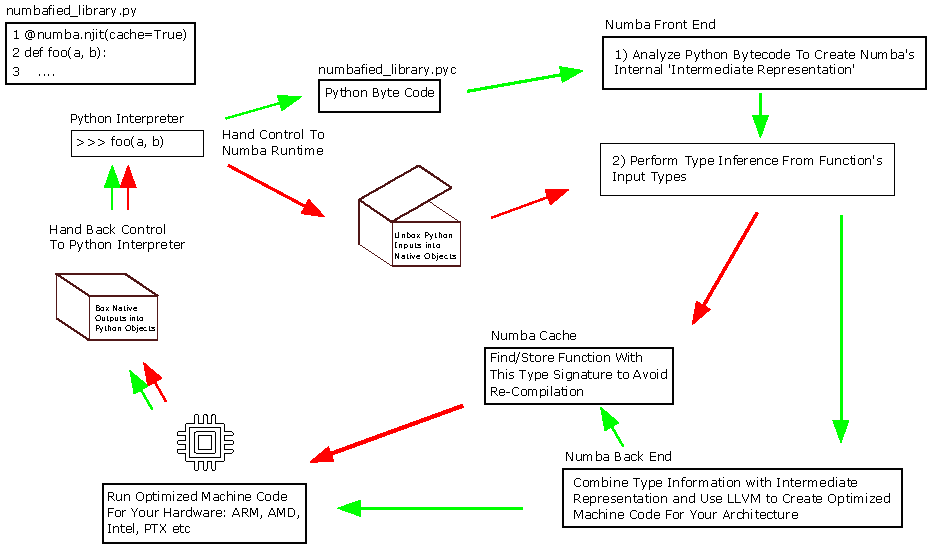
\includegraphics {figures/numba.pdf}}
    \caption{The execution path when calling a Numba compiled function from the Python interpreter. The green path is only taken if the function hasn't been called before. The red path is taken if a compiled version with the correct type signature already exists in the Numba cache.}
    \label{fig:numba}
\end{figure*}
	
\lstinputlisting[float=t, caption={An example in which loops are fused.}\label{code:loop_fusion}]{loop_fusion.py}

\lstinputlisting[float=t, caption={An example of parallel multithreading.}\label{code:parallel_multithreading}]{parallel_multithreading.py}

- Numba originally created for optimizing numpy code in loops: (1) removes indirection here -> need to know that it uses LLVM to produce a low level representation (2) can fuse together multiple loops.

- How numba targets Python code that uses this data structure. Initially, it was developed to remove layers of indirection (following multiple pointers to load data) in numpy code. This is because numpy ndarray struct has stride and bounds/dim of data it contains, so can in theory load from pointers instead of following indirection. It uses the LLVM infrastructure to optimize operations on the ndarray, especially where loops are involved - can fuse them i.e. intelligently combine loops to save computations, and apply auto vectorization if available on your cpu, and multithread using openMP or intel tbb as a backend. LLVM is a generic infrastructure for targeting various hardware architecture, so Numba's design allows to also compile for GPUs.

- Scope and aim of Numba. What is it designed to do, and what isn't it designed to do. Where it can be impactful. (ndarrays, fusing loops, autovectorization and what this is via llvm)

- how numba functions interacts with python interpreter, and the explanation of boxing/unboxing and a metric for this cost. Can only think of a good metric once I have a more secure understanding of the exact interaction here.


\section{THE FAST MULTIPOLE METHOD}

The particle FMM is an approximation algorithm for $N$-body problems in which each of the particle interacts with all other particles, for example in calculating electrostatic or gravitational potentials from a set of particles. The naive computation is $O(N^2)$, however the FMM compresses groups of interactions far away from a given particle to reduce the overall complexity to just $O(N)$.

relies on six operators that are called in a a recursive loop  over an hierarchical octree data structure [refer to specific figure in sundar paper with an octree in it] \cite{Sundar2007}.

- data structure - hierarchical, non-uniform leaves, results in 4 distinct interactions. (U, V, X, W). Explanation how this is represented linearly here in order to work with Numba.
this can be illustrated with a picture. Can refer to a figure in another paper.



- upward pass - post order traversal

P2M
- parallel. loop over leaves. check potential = $O(n_l \cdot n_{crit} \cdot n_c)$ equivalent charge = $O(n_l \cdot n_e \cdot  n_c)$.

M2M
- serial. cannot parallelize over leaves, there are parallel writes to parent multipole expansion from siblings. Parallelizing over sibling leaves is hard due to linear representation of tree - have to perform expensive neighbours searches to find siblings to perform group by. equivalent charge = $O(8^l \cdot n_e \cdot n_c)$ at a given level $l$.

- downward pass - pre-order traversal

L2L. serial - interaction

M2L

S2L

P2P

Pictures:
- illustrate expansion orders for approximating in a single box?

- tree figure, and list of kernels that are compueted at each stage, and exactly what the computations involve for kernel independent fmm. Offer complexity bounds on these calculations. Contextualize the computations required of each kernel. i.e. P2P is raw multithreading performance.

- Offer analysis of where it is suitable to parallelize.

- A short note on the decision for M2l via SVD for FMM experts.

\section{DATA ORIENTED DESIGN}

- Data oriented design.
- How this is reflected in tree design
- How this is reflected in kernel design
- API design

- Software design diagram
- Minimize the impact of running code in the interpreter.

% Larger figure
\begin{figure*}
    \centerline{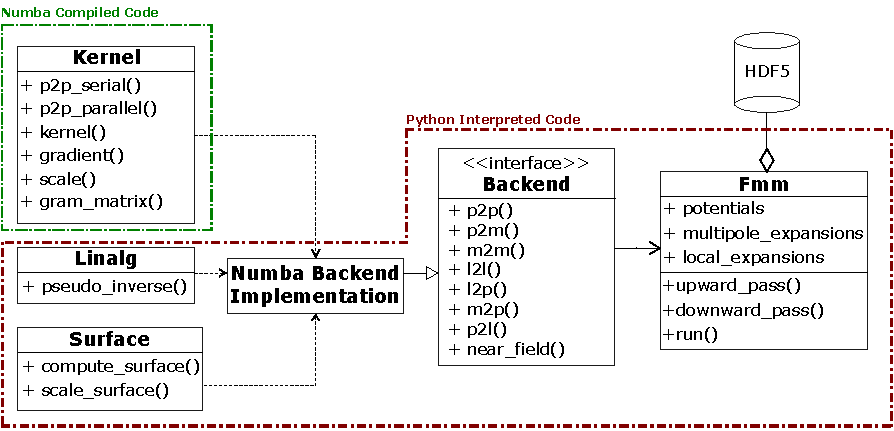
\includegraphics {figures/software.pdf}}
    \caption{Simplified UML model of all PyExaFMM components. Trees and operators are precomputed and stored in the HDF5 database. The `Fmm' object which acts as the user interface, all other components are modules consisting of methods on operating on arrays.}
    \label{fig:design}
\end{figure*}

\section{MULTITHREADING IN NUMBA}

- overview of multithreading in scientific python and the current state of affairs and why this isn't appropriate for hpc apps in pure python, and multithreading api in numba, and make analogies with openmp where they exist. Link to recent efforts to implement an OpenMP interface within Numba? 

Thread oversubscription issues and their origin and how to avoid this in Numba. Comment on the quality of this solution - the py multithreading papers from intel group have good information and experiments regarding this.

- how kernels are multithreaded bearing in mind issues raise in Numba section, and data oriented design section.
- Optimal design of multithreading approach relies on the actual constraints of the kernel in question, will need to get into specifics here of how each kernel was approached.
- metric for portion of code that is run on single vs multiple threads, can actually time this at least roughly.

\section{PITFALLS OF NUMBA}

- Numba/Numpy API differences for numerical methods can be a pitfall (svd)

- it is not Python, and writing like python (OOP) will lead to failure, numba is a framework

- not everything that is supported is fast, e.g. hashing example, and how we got around this.

- it's really designed for numerical work alone, and that's where it shines.

\section{BENCHMARKS}

- contrast multithreading impact for each kernel

- compare and contrast pyexafmm vs exafmm for a given accuracy, try and find optimum compression parameter.(?)

\section{CONCLUSION}

foo bar

\section{ACKNOWLEDGMENT}

SK is supported by EPSRC Studentship 2417009.

\bibliography{pyexafmm}

\bibliographystyle{ieeetr}

\begin{IEEEbiography}{Srinath Kailasa}{\,}is a PhD student in Mathematics at University College London. Contact him at srinath.kailasa.18@ucl.ac.uk.
\end{IEEEbiography}

\begin{IEEEbiography}{Tingyu Wang}{\,}is a PhD student in Mechanical Engineering at the George Washington University. Contact him at twang66@email.gwu.edu.
\end{IEEEbiography}

\begin{IEEEbiography}{Lorena. A. Barba}{\,}is a Professor of Mechanical and Aerospace Engineering at the George Washington University.  Contact her at labarba@email.gwu.edu.
\end{IEEEbiography}

\begin{IEEEbiography}{Timo Betcke}{\,}is Professor of Computational Mathematics at University College London. Contact him at t.betcke@ucl.ac.uk.
\end{IEEEbiography}

\end{document}

